\section{Composition---Delayed Generalization without Systematicity}

\label{sec:composition}

We begin our investigation with \textit{composition}, where a model needs to ``chain'' different pieces of facts, e.g., \textit{``Barack's wife is Michelle''} and \textit{``Michelle is born in 1964''}, to successfully complete a compositional sentence, e.g., \textit{``Barack's wife is born in [1964]''}. Prior work extensively studied whether transformer-based language models can perform implicit composition, and negative results are consistently reported~\citep{press-etal-2023-measuring, allenzhu2023physics, yang2024large}. Specifically, there exists a \textit{``compositionality gap''}~\citep{press-etal-2023-measuring}, i.e., the frequency at which the model knows all the underlying basic facts but fails to compose them, which is considerable across different LLMs and does not decrease as models scale. Are transformers doomed to fail on such kind of reasoning, and if so, why?

\subsection{Setup}
We focus on two-hop composition in this work. For atomic facts, we generate a random knowledge graph $\mathcal{G}$ consisting of $|\mathcal{E}|$ entities and $|\mathcal{R}|=200$ relations, where each entity (as the subject) has \num{20} random distinct relations that each connects to another random entity (as the object). The atomic facts are then the edges, i.e., \textit{(subject, relation, object)} triplets in $\mathcal{G}$, which we partition disjointly into \ttsmall{atomic$_{\text{ID}}$} and \ttsmall{atomic$_{\text{OOD}}$} (\num{95}\%: \num{5}\%). The rule of (two-hop) composition is
\begin{equation}
    \forall h,b,t\in \mathcal{E}, \forall r_1,r_2\in \mathcal{R}, (h,r_1,b) \land (b,r_2,t) \implies (h,r_1,r_2,t),
\end{equation}

which is used to deduce the ID and OOD inferred facts from \ttsmall{atomic$_{\text{ID}}$} and \ttsmall{atomic$_{\text{OOD}}$}, respectively. For convenience, in the above rule, we will call $h$ the \textit{head} entity, $b$ the \textit{bridge} entity, and $t$ the \textit{tail} entity. For both atomic and inferred facts, training/testing is done by having the model predict the final tail entity. We assign a unique token to each relation/entity by default, and also find that the results are robust to different tokenizations (details in Appendix~\ref{app:tokenization}).

We study the influence of the following two aspects on the model's learned behaviors:   
\begin{itemize}[noitemsep,nolistsep,leftmargin=*]
    \item \textbf{Ratio between inferred and atomic facts.} By varying the amount of inferred facts included in training, we study the effect of the ratio $\phi=|\text{\ttsmall{train\_inferred$_{\text{ID}}$}}|/|\text{\ttsmall{atomic$_{\text{ID}}$}}|$ on the model.
    \item \textbf{Training data size.} We study the impact of the training data size by varying $|\mathcal{E}|$, the total number of entities, while controlling the ratio $\phi$. Note that the size of training data (both atomic/inferred facts) scales linearly with $|\mathcal{E}|$.
\end{itemize}

\subsection{Results}

\noindent\textbf{Grokking observed in ID generalization but not in OOD generalization}. Figure~\ref{fig:grokking}(left) shows the model's accuracy on the train and test facts throughout optimization, with $|\mathcal{E}|=2000$ and $\phi=7.2$. We find that the model \textit{can} generalize to ID test examples, but high performance is only achieved through extended training far beyond overfitting, a phenomenon called \textit{grokking}~\citep{power2022grokking}. Specifically, the training performance saturates (over \num{99}\% accuracy on both atomic and inferred facts) at around 14K optimization steps, before which the highest ID generalization accuracy is merely \num{9.2}\%. However, generalization keeps improving by simply training for longer, and approaches almost perfect accuracy after extended optimization lasting around \num{50} times the steps taken to fit the training data. On the other hand, OOD generalization is never observed. We extend the training to \num{2} million optimization steps, and there is still no sign of OOD generalization.

\noindent\textbf{Inferred/atomic ratio $\phi$ correlates with generalization speed}. Figure~\ref{fig:composition}(a) shows the ID test accuracy across different $\phi$. We omit the other splits since for all settings, the training performance saturates quickly and the OOD test accuracy remains at zero as earlier.\footnote{The training performances of all settings saturate within \num{25}K steps, where larger $\phi$ takes more steps.} It could be seen that the ratio $\phi$ strongly correlates with the \textit{speed} of generalization. A very large ratio can push generalization to improve at a similar pace as the model fits the training data, reducing the need for extended training.\footnote{When $\phi=18.0$, the model achieves $96.7\%$ accuracy before training performance saturates.} 

\begin{figure}[h]
\centering
\begin{subfigure}{0.42\textwidth}
    \centering
    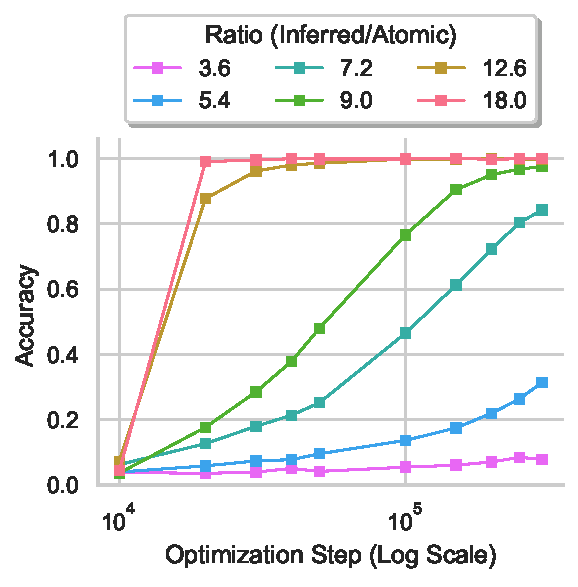
\includegraphics[width=\textwidth]{fig/ratio.pdf}
    \caption{Effect of changing ratio $\phi$ ($|\mathcal{E}|=2000$).}
\end{subfigure}
\begin{subfigure}{0.42\textwidth}
    \centering
    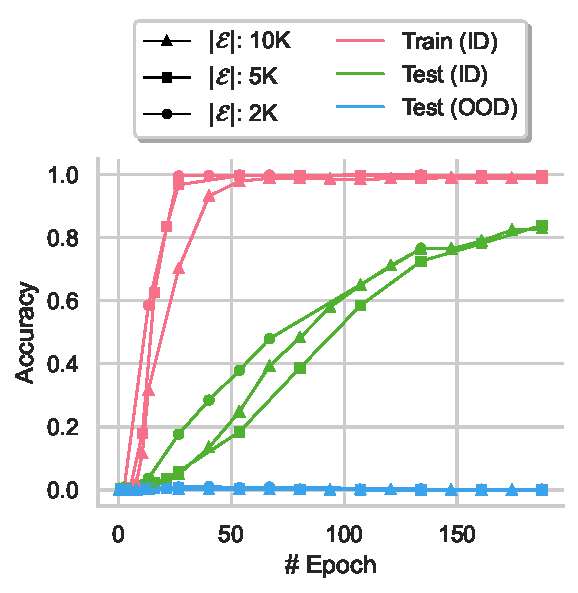
\includegraphics[width=\textwidth]{fig/size.pdf}
    \caption{Effect of changing $|\mathcal{E}|$ ($\phi=9.0$).}
\end{subfigure}
\caption{The speed of grokking on the in-distribution (ID) test performance (a) correlates with the \textit{ratio} between inferred and atomic facts, and (b) is not influenced by the \textit{size} of training data.}
\label{fig:composition}
\end{figure}

\noindent\textbf{Training data \textit{distribution}, instead of training data size, qualitatively influences generalization behavior}.
When $\phi$ increases and $|\mathcal{E}|$ holds constant, the \textit{size} of training data also gets larger. Prior studies hypothesize that training data size plays a central role in order for grokking to happen.
In particular, previous work connects grokking with the notion of \textit{critical data size} (CDS)~\citep{liu2023omnigrok, varma2023explaining, zhu2024critical, huang2024unified}, where it is hypothesized that CDS marks the shift from memorization to generalization (via grokking), and the speed of generalization improves as the training data further scales. However, results from our controlled experiments seem to contradict such a hypothesis. Figure~\ref{fig:composition}(b) shows the results of varying $|\mathcal{E}|$ with a fixed $\phi=9.0$, where we change the horizontal axis from optimization step to epoch for better visualization.\footnote{The optimization steps for each epoch scale linearly with the training size since we use a fixed batch size.} When fixing the ratio $\phi$, the training data size does \textit{not} qualitatively affect the model's generalization. Specifically, scaling the data affects neither the relative speed of ID generalization and training improvement (as seen by the rather constant ``gap'' between \ttsmall{train\_inferred$_{\text{ID}}$} and \ttsmall{test\_inferred$_{\text{ID}}$} curves), nor the systematicity level (OOD performance stays zero). We also run the experiments across different $\phi$ and find the results to be consistent. This suggests that \textit{critical data ``distribution'', not size, may be the actual deciding factor behind grokking and generalization.} In addition, we find that scaling up the model size also does not qualitatively change the generalization behaviors observed here (Appendix~\ref{app:scaling}), and the main pattern is that larger models converge in fewer optimization steps, which shares with prior findings~\citep{tirumala2022memorization, pmlr-v119-li20m}.

\noindent\textbf{Summary.} We have shown that transformers are capable of acquiring the rule of composition through grokking, with controlled experiments suggesting the crucial factor of data distribution (e.g., the inferred/atomic ratio $\phi$) in characterizing the model's generalization. However, important questions still remain: \textit{what happens during grokking, why does it happen, and why do transformers struggle with OOD examples?} Answering these questions requires a deeper understanding of (the changes in) the model's inner workings, which we investigate next.

\subsection{Analyzing the inner workings of the model throughout grokking}
\label{grokkinganalysis}

We analyze the internal mechanisms within the model via a combination of two prevalent approaches: logit lens and causal tracing. We apply our analysis to the setting with $|\mathcal{E}|=2000, \phi=9.0$ on \num{300} random examples from \ttsmall{train\_inferred$_{\text{ID}}$}.

\begin{figure}[h]
\centering
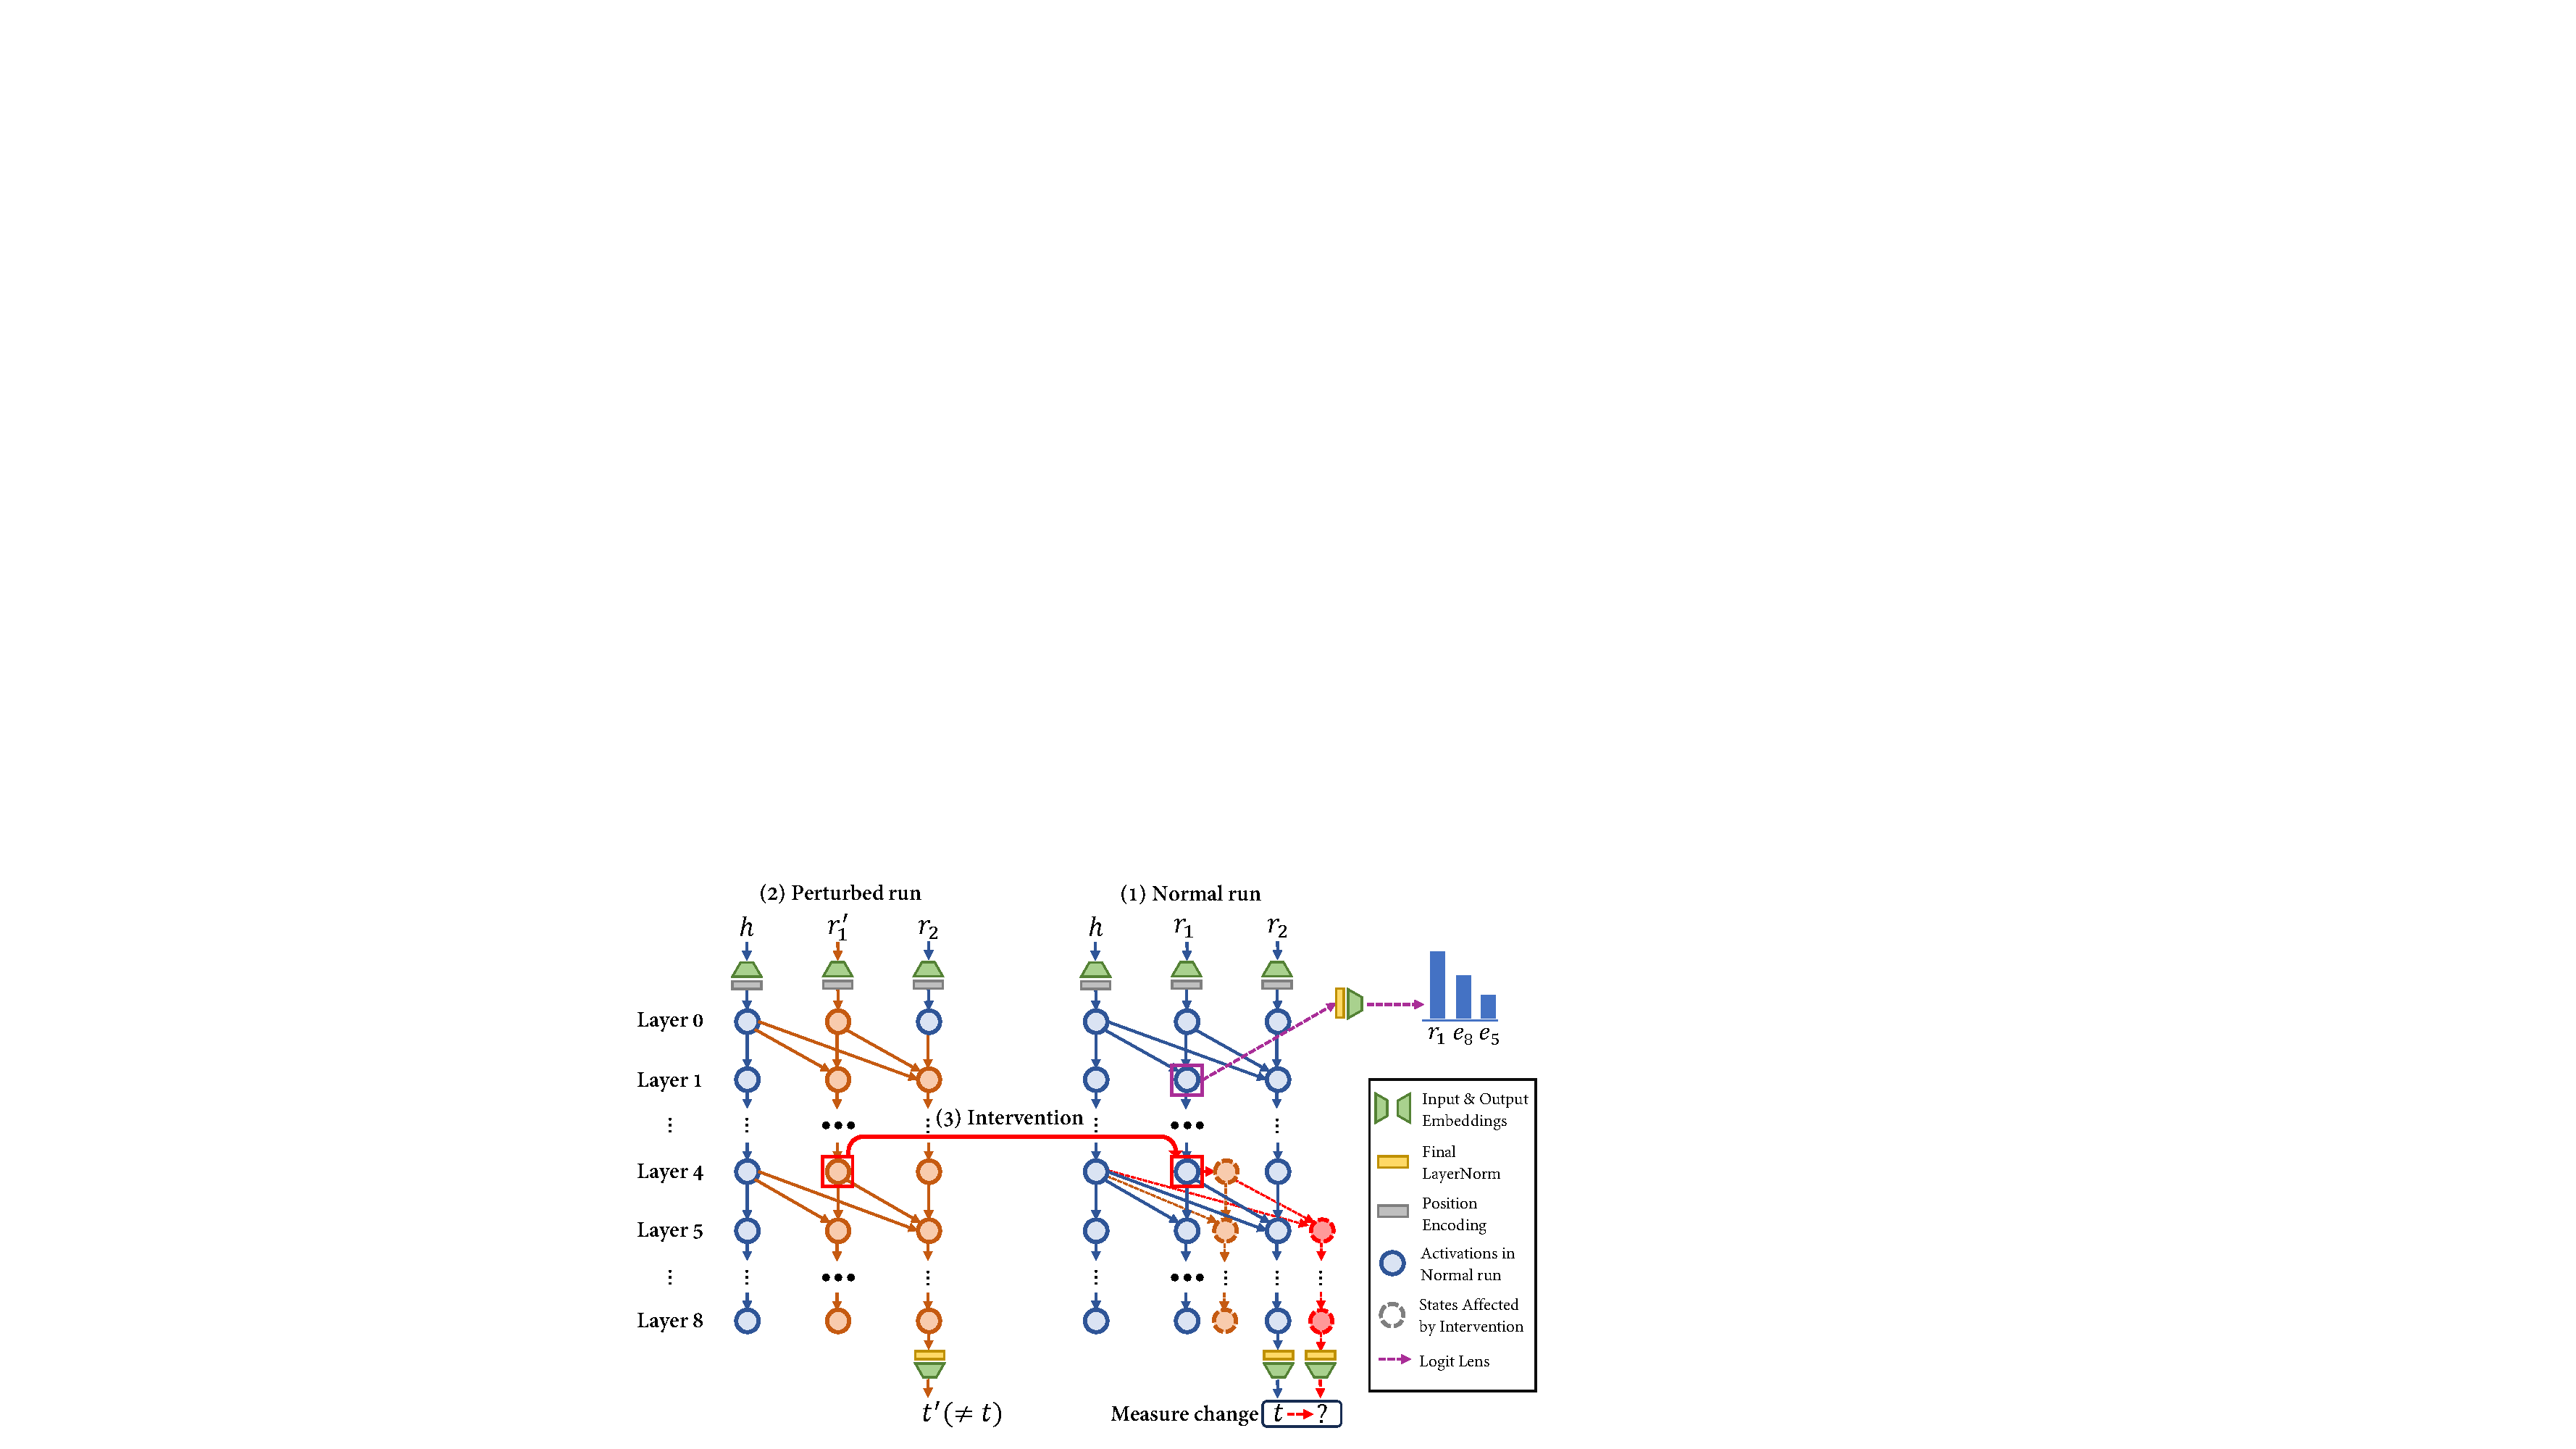
\includegraphics[width=0.77\textwidth]{fig/illustration.pdf}
\caption{Illustration of our circuit analysis approach (on the composition task). We use logit lens to interpret individual states, and use causal tracing to measure the strength of connections between states. Details are in the main content.}
\label{fig:illustration}
\end{figure}

\noindent\textbf{Logit lens}. We interpret individual hidden states via logit lens~\citep{nostalgebraist2020, geva-etal-2022-transformer, yang2024large}, where the activation is converted into a set of logits for each vocabulary token by multiplying with the output embedding matrix. We follow the recent practice~\citep{yang2024large} where the activation first goes through the transformer's final normalization layer before multiplying with the output embedding (Figure~\ref{fig:illustration}, top right). 

\noindent\textbf{Causal tracing}. The transformer could be viewed as a causal graph~\citep{pearl2009causality} that propagates information from the input to the output through a grid of intermediate states, which allows for a variety of causal analyses on its internal computations~\citep{vig2020investigating, meng2022locating, hanna2023how, wang2023interpretability, feng2024how}. For convenience, we will refer to a hidden state by $S[i,a]$, where $i$ is the layer index and $a$ marks the role of the input token at the same position as the state (one of $\{h, r_1, r_2\}$). We illustrate our method in Figure~\ref{fig:illustration}, where the hidden state of interest is $S[4,r_1]$ and the target is the model's prediction state $S[8,r_2]$. There are in total three steps:
\begin{enumerate}[noitemsep,nolistsep,leftmargin=*]
    \item The \textbf{normal run} records the model's hidden state activations on a regular input $(h,r_1,r_2)$. Note that since the model maintains perfect training performance throughout grokking, the final prediction is always the ground truth tail entity $t$.\footnote{For convenience, when we refer to a state as a token, we mean the top token of the state via logit lens.}
    \item In the \textbf{perturbed run}, a slightly perturbed input is fed to the model which changes the prediction, where again the hidden state activations are recorded. For the perturbation, prior work has explored adding noise to the input~\citep{meng2022locating} and replacing key tokens with semantically close ones~\citep{vig2020investigating, feng2024how}. We adopt token replacement which avoids unnecessary distribution shifts~\citep{zhang2024best}. Specifically, for the hidden state of interest, we replace the input token at the same position as the state to be a random alternative of the same type (e.g., $r_1\rightarrow r_1'$) that leads to a different target prediction (e.g., $t\rightarrow t'$).
    \item \textbf{Intervention}. During the normal run, we intervene the state of interest by replacing its activation with its activation in the perturbed run. We then run the remaining computations and measure if the target state (top-\num{1} token through logit lens) is altered. The ratio of such alterations (between \num{0} and \num{1}) among the examples quantitatively characterizes the \textit{causal strength} between the state of interest and the target.
\end{enumerate}

\begin{figure}[h]
\centering
\begin{subfigure}{0.38\textwidth}
    \centering
    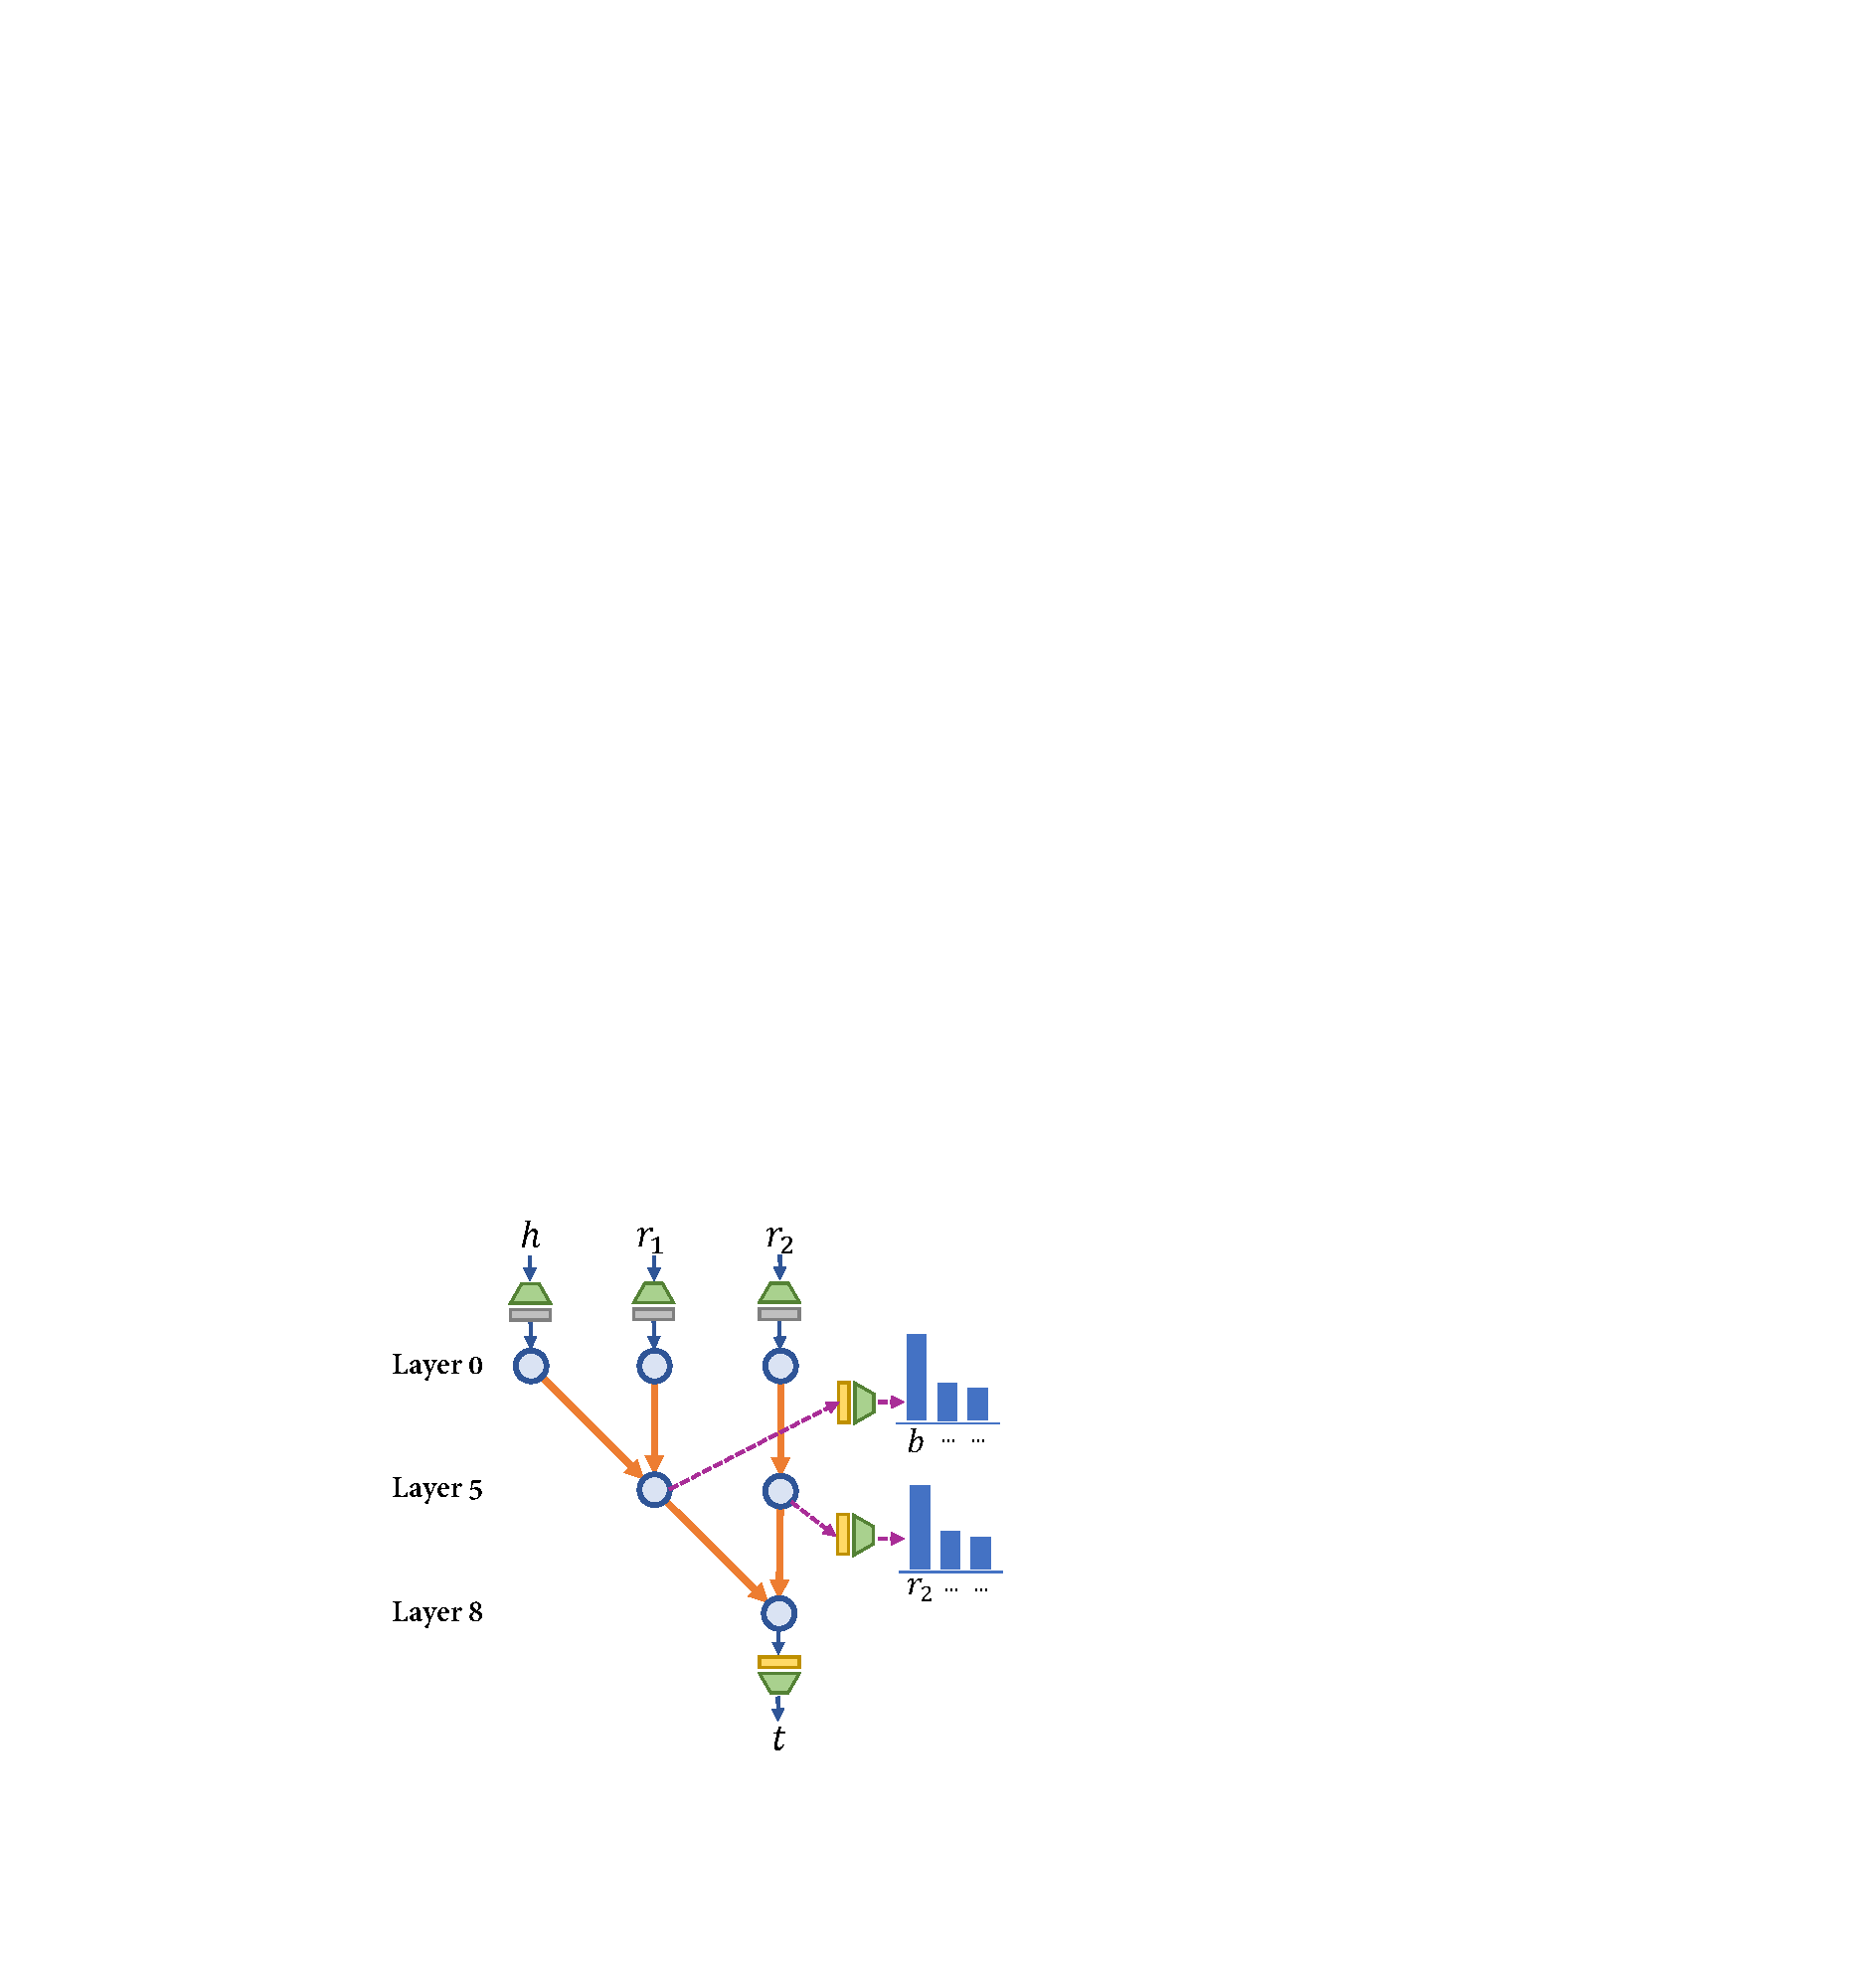
\includegraphics[width=\textwidth]{fig/circuit_composition.pdf}
    \caption{}
\end{subfigure}
\begin{subfigure}{0.25\textwidth}
    \centering
    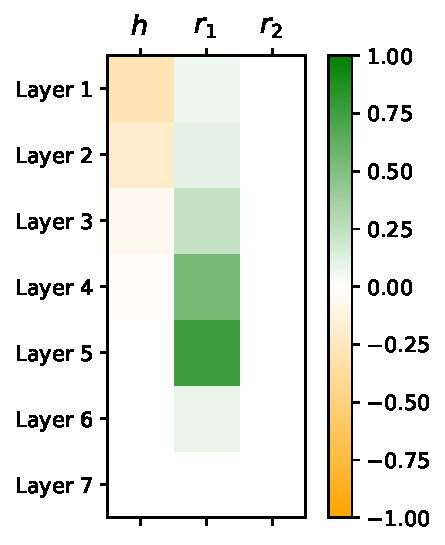
\includegraphics[width=\textwidth]{fig/causal_composition_diff.pdf}
    \caption{}
\end{subfigure}
\begin{subfigure}{0.35\textwidth}
    \centering
    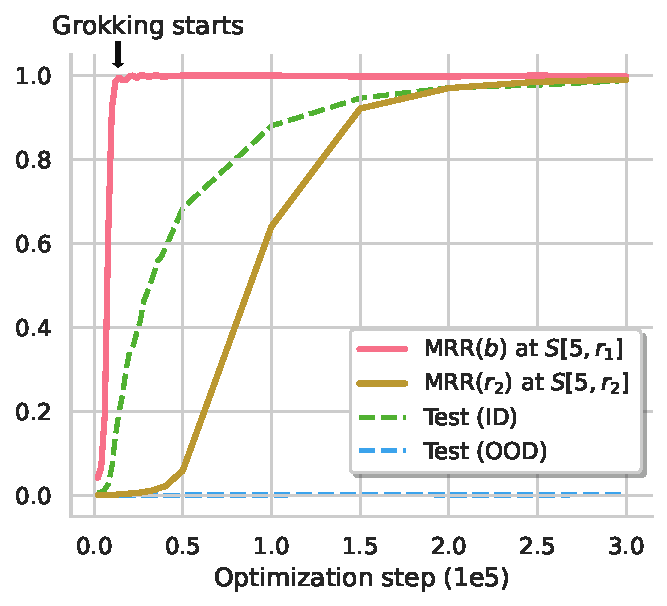
\includegraphics[width=\textwidth]{fig/MRR_composition.pdf}
    \caption{}
\end{subfigure}
\caption{The (evolution of) generalizing circuit for composition. (a) The generalizing circuit. (b) The \textit{change} in causal strengths during grokking, where the target is the prediction state. (c) Mean reciprocal rank (via logit lens) of the bridge entity $b$ at $S[5,r_1]$ and second relation $r_2$ at $S[5,r_2]$.}
\label{fig:circuit_composition}
\end{figure}

\noindent\textbf{The generalizing circuit}. We run a set of causal tracing and logit lens experiments across different model checkpoints throughout training. The discovered generalizing circuit (i.e., the causal computational pathways after grokking) is illustrated in Figure~\ref{fig:circuit_composition}(a). Specifically, we locate a highly interpretable causal graph consisting of states in layer \num{0}, \num{5}, and \num{8}, where we have pruned away the weak nodes/connections (details in Appendix~\ref{app:circuit}). Layer \num{5} splits the circuit into lower and upper layers, where 1) the lower layers retrieve the first-hop fact $(h,r_1,b)$ from the input $h,r_1$, store the bridge entity $b$ in $S[5,r_1]$, and ``delay'' the processing of $r_2$ to $S[5,r_2]$; 2) the upper layers retrieve the second-hop fact $(b,r_2,t)$ from $S[5,r_1]$ and $S[5,r_2]$, and store the tail $t$ to the output state $S[8,r_2]$.

\noindent\textbf{What happens during grokking?} To understand the underlying mechanism behind grokking, we track the strengths of causal connections and results from logit lens across different model checkpoints during grokking (the ``start'' of grokking is the point when training performance saturates). We observe two notable amplifications (within the identified graph) that happen during grokking. The first is the causal connection between $S[5,r_1]$ and the final prediction $t$, which is very weak before grokking (Appendix~\ref{app:circuit}) and grows significantly during grokking (Figure~\ref{fig:circuit_composition}(b)). The second is the $r_2$ component of $S[5,r_2]$ via logit lens, for which we plot its mean reciprocal rank (MRR) (Figure~\ref{fig:circuit_composition}(c)). Additionally, we find that the state $S[5,r_1]$ has a large component of the bridge entity $b$ throughout grokking (Figure~\ref{fig:circuit_composition}(c)). These observations strongly suggest that the model is \textit{gradually forming the second hop in the upper layers (\num{5}-\num{8}) during grokking}.
This also indicates that, before grokking, the model is very likely mostly memorizing the examples in \ttsmall{train\_inferred$_{\text{ID}}$} by \textit{directly associating $(h,r_1,r_2)$ with $t$}, without going through the first hop.

\noindent\textbf{Why does grokking happen?} These observations suggest a natural explanation of why grokking happens through the lens of circuit efficiency~\citep{varma2023explaining}.
Specifically, as illustrated above, there exist both a memorizing circuit $C_{mem}$ and a generalizing circuit $C_{gen}$ that can fit the training data. While $C_{mem}$ is learned first (which causes training performance to saturate quickly), $C_{gen}$ is relatively more \textit{efficient}, in the sense that it could fit the data with a lower complexity.
To see this, we can compare the amount of facts $C_{mem}$ and $C_{gen}$ need to store (denoted as $N_{mem}$ and $N_{gen}$) as a proxy for their complexity.\footnote{While the circuits also consist of other components, they pale in comparison as the number of facts scales.}
$C_{mem}$ stores both atomic facts and inferred facts in the weights. $C_{gen}$ (Figure~\ref{fig:circuit_composition}(a)) stores the atomic facts in the lower layers, and another copy of the atomic facts that \textit{appear as the second hop in the inferred facts} in the upper layers. As the inferred/atomic ratio $\phi$ increases, $N_{mem}$ would increase rapidly while $N_{gen}$ increases slowly and is always bounded by two times the total amount of atomic facts, and hence, the relative efficiency of $C_{gen}$ increases. In the long run, the model will be incentivized to transition from $C_{mem}$ to $C_{gen}$ due to implicit bias of the optimization~\citep{soudry2018the} and explicit regularization such as weight decay which prefers more efficient circuits, and the transition would happen faster as $\phi$ increases. This also explains why the training data size does not affect the speed of grokking, since \textit{solely increasing the size does not change the relative efficiency of $C_{mem}$ and $C_{gen}$}. The explanation also implies that a larger regularization factor should accelerate grokking (and vice versa), which we confirm by varying the degree of weight decay (Appendix~\ref{app:wd}).

\noindent\textbf{Explaining and mitigating the deficiency in OOD generalization.} The configuration of $C_{gen}$ also has another important implication: while the model does acquire compositionality through grokking, it \textit{does not have any incentive to store atomic facts in the upper layers that do not appear as the second hop during training}. This explains why the model fails in the OOD setting where facts are only observed in the atomic form, not in the compositional form---the OOD atomic facts are simply not stored in the upper layers when queried during the second hop.\footnote{We verified that in the OOD setting, $S[5,r_1]$ and $S[5,r_2]$ encode $b$ and $r_2$ respectively as in the ID case.} Such issue originates from the non-recurrent design of the transformer architecture which forbids memory sharing across different layers. Our study provides a mechanistic understanding of existing findings that transformers seem to reduce compositional reasoning to linearized pattern matching~\citep{dziri2023faith}, and also provides a potential explanation for the observations in recent findings that LLMs only show substantial positive evidence in performing the first hop reasoning but not the second~\citep{yang2024large}. Our findings imply that proper cross-layer memory-sharing mechanisms for transformers such as memory-augmentation~\citep{sukhbaatar2015end, graves2016hybrid} and explicit recurrence~\citep{dehghani2018universal, hutchins2022blockrecurrent, tan-etal-2023-sparse} are needed to improve their generalization. We also show that a variant of the parameter-sharing scheme in Univeral Transformer~\citep{dehghani2018universal} can improve OOD generalization in composition (Appendix~\ref{app:ut}).